\section{Procedure}
\label{sec:procedure}
The optical arrangement is sketched in \autoref{fig:setup} and will be explained in the following
paragraphs.

\begin{figure}
  \centering
  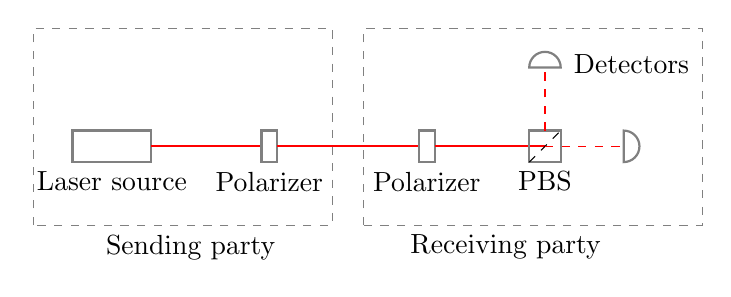
\begin{tikzpicture}
    \draw[gray, thick] (-3.5,-0.2) rectangle (-2.5,0.2); 
    \node[below] at (-3,-0.2) {Laser source};
    \draw[red, thick] (-2.5,0) -- (-1.1,0); 

    \draw[gray, thick] (-1.1,-0.2) rectangle (-0.9,0.2); 
    \node[below] at (-1,-0.2) {Polarizer};

    \draw[red, thick] (-0.9,0) -- (0.9,0); 

    \draw[gray, thick] (0.9,-0.2) rectangle (1.1,0.2); 
    \node[below] at (1,-0.2) {Polarizer};

    \draw[red, thick] (1.1,0) -- (2.5,0); 
    \draw[gray, thick] (2.3,-0.2) rectangle (2.7,0.2); 
    \draw[dashed] (2.3,-0.2) -- (2.7,0.2);
    \node[below] at (2.5,-0.2) {PBS};

    \draw[gray, thick] (2.3,1) -- (2.7,1) arc(0:180:0.2) --cycle;

    \draw[gray, thick] (3.5,0.2) -- (3.5,-0.2) arc(-90:90:0.2) --cycle;
    \node[above] at (3.6,0.8) {Detectors};

    \draw[red, dashed] (2.5,0.2) -- (2.5,1);
    \draw[red, dashed] (2.5,0) -- (3.5,0);

    \draw[gray, thin, dashed] (-4,-1) rectangle (-0.2,1.5);
    \node[below] at (-2,-1) {Sending party};

    \draw[gray, thin, dashed] (0.2,-1) rectangle (4.5,1.5);
    \node[below] at (2,-1) {Receiving party};
  \end{tikzpicture}
    \caption{Optical setup to test the BB84 protocoll with light polarization states. The intensity
      of each light
      beam after passing the polarizing beam splitter (PBS) depends on the two polarizer settings and
  the initial polarization of the laser.}
  \label{fig:setup}
\end{figure}
